%************************************************
\chapter{Models of Cognition Introduction}\label{ch:models_of_cognition_introduction}
%************************************************

\begin{quote}
Problem-solvers must find relevant data.  How does the human mind
retrieve what it needs from among so many millions of knowledge items?
Different AI systems have attempted to use a variety of different
methods for this.  Some assign keywords, attributes, or descriptors to
each item and then locate data by feature-matching or by using more
sophisticated associative data-base methods.  Others use
graph-matching or analogical case-based adaptation.  Yet others try to
find relevant information by threading their ways through systematic,
usually hierarchical classifications of knowledge---sometimes called
``ontologies''.  But, to me, all such ideas seem deficient because it
is not enough to classify items of information simply in terms of the
features or structures of those items themselves.  This is because we
rarely use a representation in an intentional vacuum, but we always
have goals---and two objects may seem similar for one purpose but
different for another purpose.
\end{quote}
\begin{flushright}
 --- \defcitealias{minsky:1991}{Marvin Minsky}\citetalias{minsky:1991}
\end{flushright}

\section{The Agent Environment Model}

\begin{figure}[bth]
  \center
  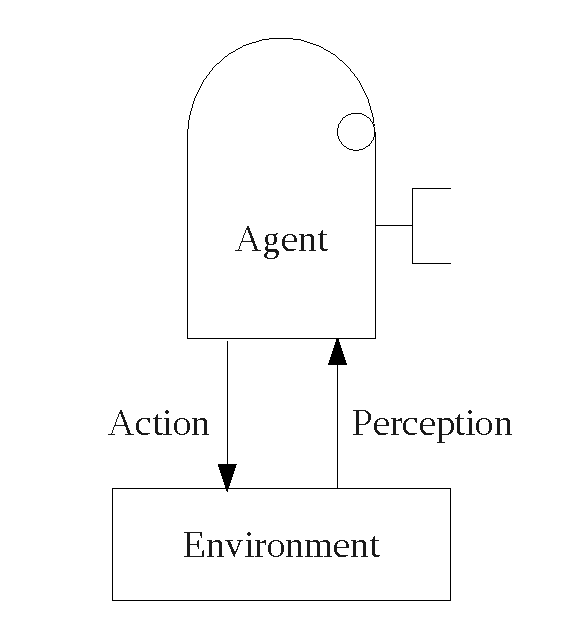
\includegraphics[height=5cm]{gfx/agent_environment}
  \caption[The agent environment model]{The agent environment model.}
  \label{fig:agent_environment}
\end{figure}

Figure~\ref{fig:agent_environment} shows the basic agent environment
model.  In this model, we make a distinction between the environment
and the agent.  At any given time, the agent and the environment are
each represented as a specific static form of data.  Further, these
representations change over time, according to a given transfer
function.  We will treat this system as a deterministic system,
although one could imagine adding random variables to the transfer
function: the basic theory is the same.  It is easier to add
randomness to a deterministic theory than the opposite.  There are
also many benefits to developing a deterministic model with perhaps a
pseudorandom aspect because this allows for the repeatability of
scientific experiments, for which the model may be used as a metric.
The two processes communicate information along two channels: (1) an
action channel from the agent to the environment, and (2) a perception
channel from the environment to the agent.

\section{The Multiple Agent Environment Model}

\begin{figure}[bth]
  \center
  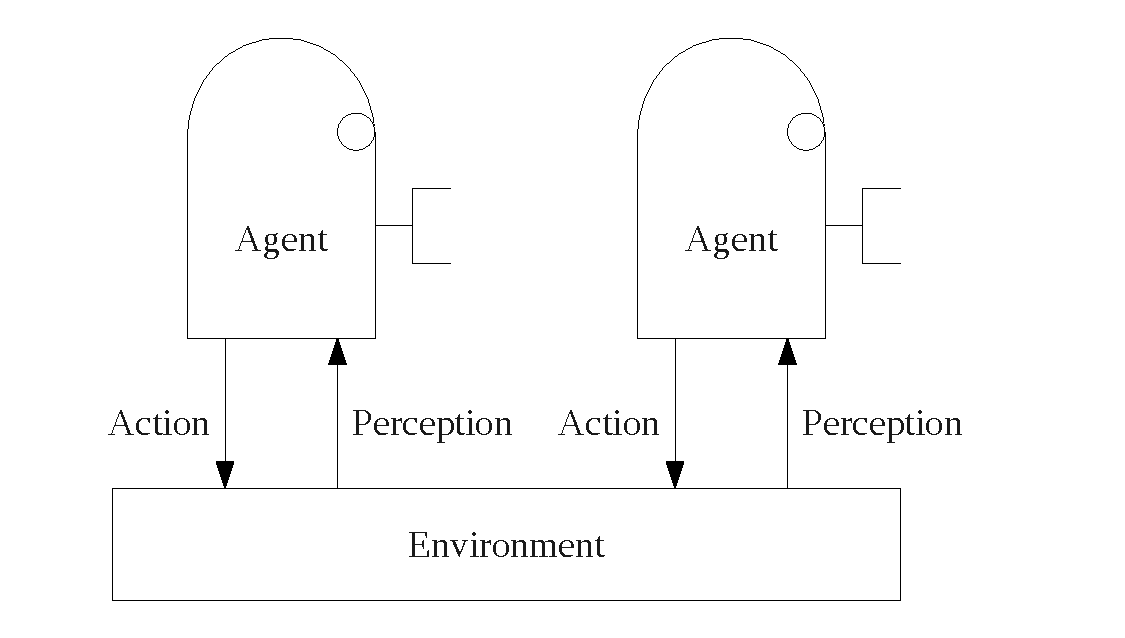
\includegraphics[height=5cm]{gfx/multiple_agent_environment}
  \caption[The multiple agent environment model]{The multiple agent environment model.}
  \label{fig:multiple_agent_environment}
\end{figure}

In order to model social intelligence, we introduce the multiple agent
environment model shown in
Figure~\ref{fig:multiple_agent_environment}.  One interesting property
of the multiple agent environment model is that any communication
between any two agent processes must occur through the environment
process.


\section{The Baby-Machine Approach}

\subsection{The Reinforcement Learning Model}

\begin{figure}[bth]
  \center
  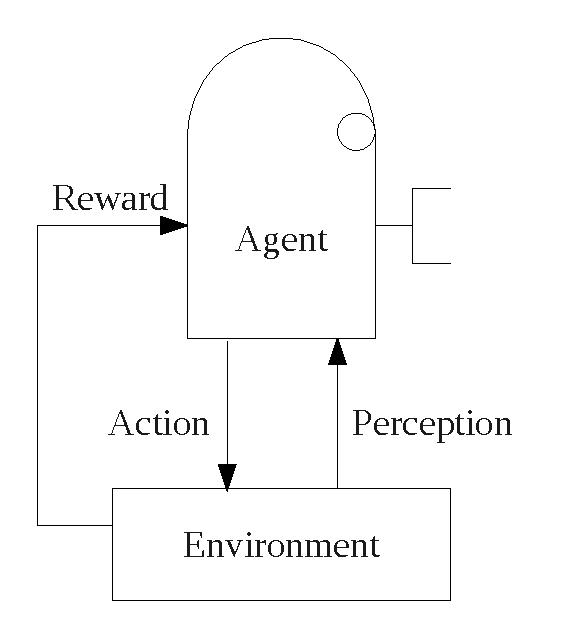
\includegraphics[height=5cm]{gfx/reinforcement_learning}
  \caption[The reinforcement learning model]{The reinforcement learning model.}
  \label{fig:reinforcement_learning}
\end{figure}

Figure~\ref{fig:reinforcement_learning} shows the basic reinforcement
learning model.  This model is an agent environment model, but there
is an extra information channel from the environment to the agent,
which communicates a numerical reward signal.  We can now say that the
agent has a learning problem.  The agent must learn what actions to
execute in order to gather the most reward.

\begin{figure}[bth]
  \center
  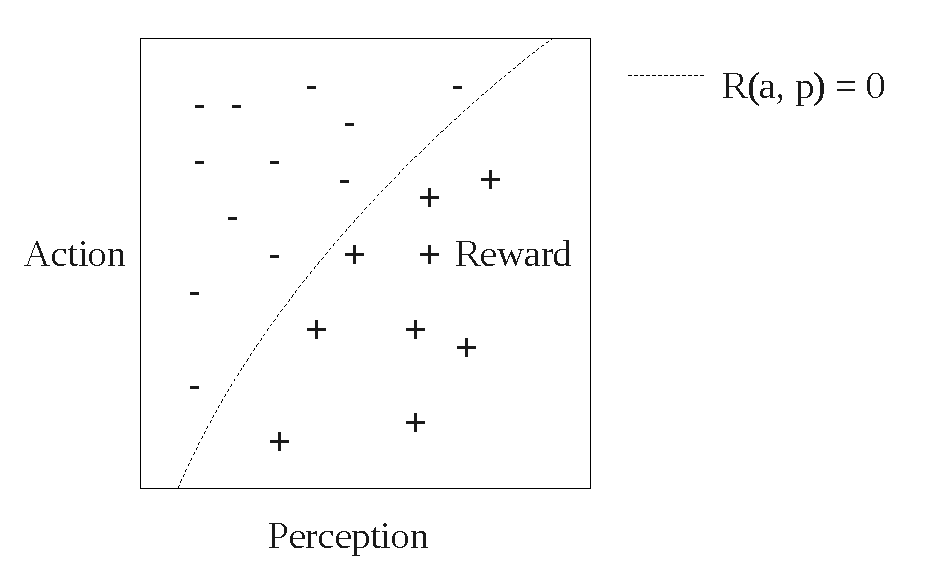
\includegraphics[height=4cm]{gfx/perception_categorization}
  \caption[Categorizing perceptions and actions based on goals]{Categorizing perceptions and actions based on goals.}
  \label{fig:perception_categorization}
\end{figure}

Once we have a basic reinforcement learning algorithm, we can approach
this learning problem as a function approximation problem.  In other
words, we can try to learn what parts of the perception and action
space have more or less reward.
Figure~\ref{fig:perception_categorization} shows a diagram of this
state space with the zero crossing of an approximation of the reward
plotted.

\subsection{Finding a Good Policy for Gathering Rewards}

Learning an approximation of what parts of a state space are good or
bad, based on reward, is not all that is needed to determine what
actions the agent should perform.  The agent wants to gather the most
rewards over time.  A simple way to formalize this problem is to learn
a policy that determines what action should be executed for every part
of the state space, based on some sort of summation of rewards over
time.  There have a been a number of ways of formalizing this
summation process as finite or infinite horizon problems
\citep{sutton:1998}.  Dynamic programming can be used for finding an
optimal or an approximately optimal policy \citep{bertsekas:1995}.

\subsection{Categorizing Perceptions and Actions based on Goals}

One problem with the reinforcement learning approach is that the only
representation of success or failure is a single number, the reward.
The basic reinforcement learning problem has been defined for finite
propositional state spaces.

A representation called \ac{RMDP} has been proposed
\citep{guestrin:2003} in order to extend reinforcement learning to
larger relational problem domains, but this method only focuses on an
object-oriented reward that does not have any global feedback about
the overall value of the situation.


\subsection{Feedback Control Model for Accomplishing Goals}

\begin{figure}[bth]
  \center
  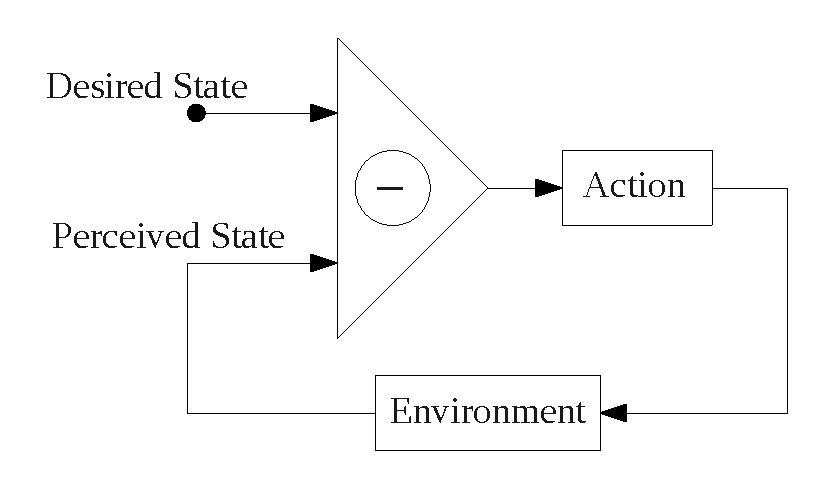
\includegraphics[width=6cm]{gfx/feedback_control}
  \caption[The feedback control model for accomplishing goals]{The feedback control model for accomplishing goals.}
  \label{fig:feedback_control}
\end{figure}

Now that we have discussed the basic model of learning from experience
what good goal states may be from rewards, let us consider the
representations for the state space of the perceptions and actions of
our model.  Control theory has given us many useful models for agents
that control continuous environments.  For example,
Figure~\ref{fig:feedback_control} shows a simple difference feedback
control circuit that is used in simple linear control systems.  The
system is given a desired state, there is a difference device that
calculates the difference between the actual perceived value from the
environment, and the control system then executes an action based on
that difference, which affects the environment.  The result in such a
negative feedback loop is that the agent's perception of the
environment is closer to the desired state.

\subsection{Means-End Analysis}

In 1959, Newell, Shaw, and Simon published a report on a means-end
analysis model that was designed to solve any symbolically represented
problem \citep{newell:1959}.  Their system was called the \ac{GPS}, and
worked by being able to work with relational representations of
current and desired states.  The agent had a catalogue of differences
between states that it knew how to minimize.  The system worked by
finding the largest difference and executing the associated method for
reducing this difference.  This work has grown into the Soar model for
better solving symbolic planning problems, and dealing with impasses
for when the planning search runs out of options.




\subsection{Goal-Oriented Learning}



\section{The Origins of Knowledge}

If we are going to be clear about what we mean by meta-knowledge, we
first must be more precise about what we mean by knowledge in the
first place.


\section{Layers of Knowledge about Knowledge}




\section{Two Popular Approaches to Modelling Intelligence}

Recently, there have been two directions of research with the goal of
building a machine that explains intelligent human behavior.  The
first approach is to build a baby-machine that learns from scratch to
accomplish goals through interactions with its environment.  The
second approach is to give the machine an abundance of knowledge that
represents correct behavior.

Each of these solutions has benefits and drawbacks.  The baby-machine
approach is good for dealing with novel problems, but these problems
are necessarily simple because complex problems require a lot of
background knowledge.  The data abundance approach deals well with
complicated problems requiring a lot of background knowledge, but
fails to adapt to changing environments, for which the algorithm has
not already been trained.

\subsection{Adaptability in Complex Environments}

\begin{figure}[bth]
  \center
  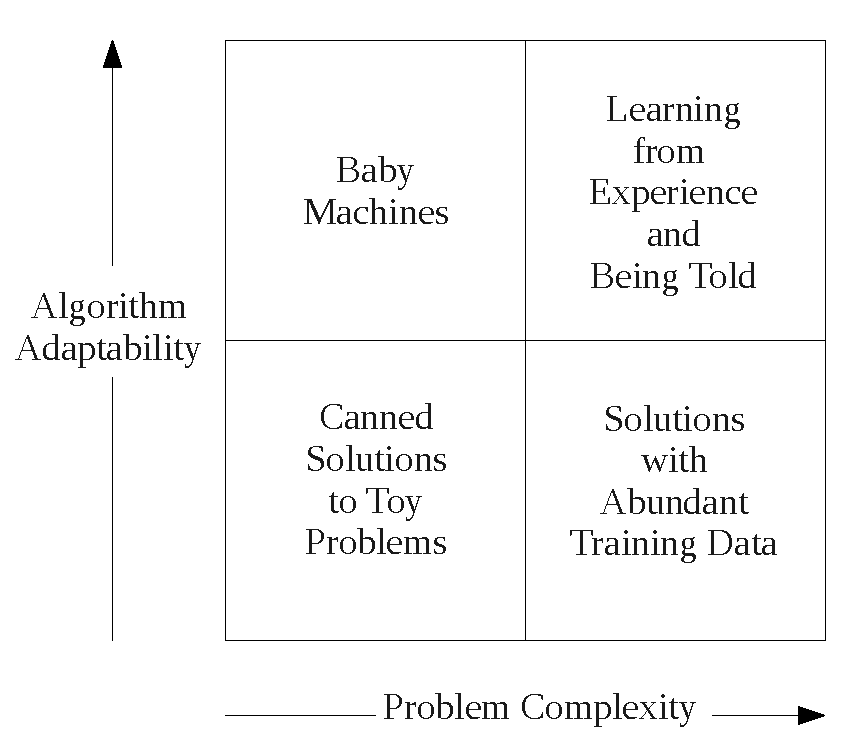
\includegraphics[height=6cm]{gfx/problem_complexity_versus_algorithm_adaptability}
  \caption[Problem complexity versus algorithm adaptability]{Problem
    complexity versus algorithm adaptability.}
  \label{fig:problem_complexity_versus_algorithm_adaptability}
\end{figure}

We would like to build intelligent machines that are able to perform
household tasks, such as cooking, cleaning, and doing the laundry, but
these tasks seem insurmountably complex, containing organically
unpredictable events.  We would like our machines to expertly handle
these extremely complicated problems, and we would also like them to
adapt to learn in unexpected or novel situations.  One popular
approach to building a machine that performs complicated tasks is to
give the machine a large training dataset that details every possible
situation that the machine may find itself within, along with the
correct action in that situation.  This is the so-called
``supervised'' learning approach.  These algorithms do not adapt to
novel situations well, and collecting these datasets is often
impossible for many problems, such as cooking and cleaning because it
is too difficult to enumerate all possible situations, in which the
machine may find itself.  Also, if the machine is cooking a meal, we
would like to be able to explain an idea for a new recipe to the
machine, or to perhaps be a partner in discovering new recipes, or we
may simply want to explain to the machine that a guest has a specific
allergy to walnuts, making that ingredient an exception for this meal
but not others.
Figure~\ref{fig:problem_complexity_versus_algorithm_adaptability}
shows how problem complexity and algorithm adaptability can be thought
of as a two-dimensional space into which different algorithmic
approaches can be used as solutions.

\subsection{The Abundant Data Approach}

There have been many approaches to modelling complex forms of
reasoning by collecting large amounts of knowledge that describes
correct or acceptable behavior in a domain.  For example, there are
examples of complex multi-agent commonsense simulation environments
collects thousands of examples of users interacting in a complicated
object-oriented social simulation \citep{orkin:2009},
\citep{orkin:2010}.  These systems have complicated domains, but these
projects do not attempt to build agents that attempt to accomplish
goals.  Instead, these systems are inference systems that simply try
to reproduce typical behavior, rather than goal-directed behavior.

There are many commonsense reasoning systems that do not interact with
simulation environments at all, but which attempt to demonstrate
commonsense reasoning by being told large amounts of knowledge.  The
Cyc project is one large such project that has been told large amounts
of logical knowledge \citep{lenat:1990}.  There is also effort
directed toward populating Cyc with knowledge automatically gathered
from the web \citep{matuszek:2005}.  The OpenMind project
\citep{singh:2002} is a project that gathers large amounts of
approximately correct commonsense knowledge from people online.  The
OpenMind knowledge has been turned into many inference systems that
can compare and generate new commonsense knowledge \citep{liu:2004a,
  liu:2004b, speer:2008}.

\section{The Common Sense Reasoning Problem Domain}

Common sense is the set of common reasoning abilities shared by most
people in a given social group.  Another way to say this is that
common sense is the set of reasoning abilities that one would assume
of a typical person that they meet for the first time and know nothing
about.  For example, most people have a naive theory of physics, so
you would expect someone to know that things fall when they are not
supported and liquids flow or are absorbed unless they are in a
container.  Common sense relies on a lot of knowledge that is assumed
that most everyone knows.

%TS>> what is a given social group... i share very little reasoning abiltities about user TS>>interface with my daughter or the director of CMU Siliicon Valley or my bike riding 
%TS>> friends, or my brothers,....

%TS>> not crisp enough ... a person is not defined as a person...but realtive to a 
%TS>> role we have with them,,, a mechanic talks differently to a woman or man, a professor
%TS>> or his accountant about cars 

%TS>> again, people have different theories of physics than each other 

%TS>> i have been served food in which the floating stuff  was designed to change through 
%TS>> the period of servign and eating soup  ..

%TS>> I am ready for  a fight on that , i live with a woman, a teenage girl, an autistic,
%TS>> my neighbor is a morman, the woman next door is totally rich... very diffferent 
%TS>> world views... even about how to deal with trash from a dinner. 

%TS>> I don't know what YOU mean by common sense yet,,,, define something specific
%TS>> does it cover diffferent minds or clones, what about its edges,   


Building a machine that demonstrates common sense reasoning is a
long-standing goal of the field of artificial intelligence.  One of
the difficulties in developing algorithms for dealing with a common
sense reasoning domain is that the algorithm needs a lot of background
knowledge about a given domain before it can answer even simple
questions about it.  However, this knowledge is often only true in
very specific situations and has many exceptional cases.  For example,
the knowledge that most birds can fly is generally true, but we also
know that many birds are flightless, such as penguins, ostriches, and
road runners.  Also, we have knowledge about the typical behavior of
objects; for example, we know that refrigerators keep things cold,
but we also reason efficiently about exceptional cases, such as when
the refrigerator is not plugged in, or when the power goes out.

%TS>> yes but those are examples we have seen for decades with varying 
%TS>> logical relations solving them
%TS>> show some that we haven't been able to do or places where you hold
%TS>> up where others have always been brittle 
%TS>> flexibility, integrity, hypocracy, intentionality changing belief systems...? 


\subsection{Representations for Common Sense Reasoning}

There have been many approaches to artificial intelligence that use
first-order logic as a representation for these types of knowledge and
their exceptions, but these systems become cumbersome in their
inability to express ``fuzzy'' sorts of relationships, such as when
the knowledge is applicable, for example the modifiers, ``most of the
time'', ``usually'', and ``almost never'', are difficult to express in
first-order logic.  When we have a lot of knowledge, we need ways to
keep track of in which situations this knowledge is useful.  This is a
form of ``meta-knowledge'', or knowledge about knowledge.
Meta-knowledge about first-order logic cannot be expressed in
first-order logic, so another type of representation is required for
this type of knowledge.  Therefore, we need other ways to represent
our knowledge in addition to logic.

\begin{quote}
``Nonetheless, theorem proving is in the worst case an intractable
  problem, even with no variables or unification, so no algorithm is
  going to work on the problem all the time. In this respect, theorem
  proving, for all its superficial formalism, is a lot like other
  branches of AI.  Where a theorist views a problem as solved if he
  has found an efficient algorithm or a discouraging lower bound, an
  AI researcher is often happy to find an algorithm that seems to work
  on some interesting problems, even though he doesn't really know the
  bounds of what it can do. Exploration will reveal the extent of its
  powers-each time it solves one more interesting problem something
  has been
  gained.''~---~\defcitealias{mcdermott:1987}{Drew~McDermott}\citetalias{mcdermott:1987}
\end{quote}


